% !TEX program = xelatex
% !TeX encoding = utf8
% !TeX spellcheck = pl-PL

%%%%%%%%%%%%%%%%%%%%%%%%%%%%%%%%%%%%%%%%%%%%%%%%%%%%%%%%%%%%%%%%%%%%%%%%%%%
% Wybierz rodzaj pracy dyplomowej oraz wydział
% Pick thesis type and faculty
%%%%%%%%%%%%%%%%%%%%%%%%%%%%%%%%%%%%%%%%%%%%%%%%%%%%%%%%%%%%%%%%%%%%%%%%%%%
\documentclass[thesis=inz,faculty=ee]{EE-dyplom} 

% thesis=[inz|mgr|bsc|msc]
%  * inz - praca inżynierska
%  * mgr - praca magisterska
%  * bsc - bachelor thesis
%  * msc - master thesis

% Skróty nazw wydziałów zgodne z domenami internetowymi
% Abbreviations of Faculties according to Internet subdomains
% faculty=[
%	arch,
%	gik,
%	ee,
%	wip
%	]

%%%%%%%%%%%%%%%%%%%%%%%%%%%%%%%%%%%%%%%%%%%%%%%%%%%%%%%%%%%%%%%%%%%%%%%%%%%
% Konfiguracja - do personalizacji
% Configuration - to be personalized
%%%%%%%%%%%%%%%%%%%%%%%%%%%%%%%%%%%%%%%%%%%%%%%%%%%%%%%%%%%%%%%%%%%%%%%%%%%
\instytut{Instytut Elektrotechniki Teoretycznej i Systemów Informacyjno-Pomiarowych}
\kierunek{Informatyka Stosowana}
\specjalnosc{Inżynieria danych i multimedia}
\title{Konstrukcja i oprogramowanie robota wyposażonego w kamerę do monitorowania budynku}
\engtitle{Constructing and programming a camera equipped robot for indoor surveillance}
\album{319084}
\author{Jordan Parviainen}
\promotor{dr hab. inż. Marcin Kołodziej, prof.}
\date{2025}
\longdate{2025-02-06}

%\grantlicense{TRUE} % [TRUE|FALSE]

%%%%%%%%%%%%%%%%%%%%%%%%%%%%%%%%%%%%%%%%%%%%%%%%%%%%%%%%%%%%%%%%%%%%%%%%%%%
% Streszczenie pracy i abstract.
% In case of thesis in English swap the order - English version goes first.
%%%%%%%%%%%%%%%%%%%%%%%%%%%%%%%%%%%%%%%%%%%%%%%%%%%%%%%%%%%%%%%%%%%%%%%%%%%
\streszczeniepracy{
Praca dotyczy konstrukcji i oprogramowania mobilnego robota wyposażonego w kamerę, wykorzystującego Raspberry Pi jako platformę sprzętową.
Celem pracy było stworzenie funkcjonalnego zdalnie sterowanego robota, który może być wykorzystany do monitorowania budynku.

We wstępie przedstawiono cel i zakres pracy, jak i motywację wyboru tematyki.
Przybliżono problematykę nowoczesnych metod monitoringu i zaprezentowano istniejące rozwiązania naukowe oraz komercyjne.

W kolejnej części opisano sprzęt, który został użyty do zbudowania robota.
Opisano wykorzystane elementy konstrukcyjne -- gotowy zestaw podwozia z silnikami elektrycznymi.
Przedstawiono nakładkę Motor Driver Hat, która pozwala na sterowanie silnikami i zasilanie Raspberry Pi.
Opisano również zasilanie akumulatorowe, które zastosowano w robocie.
Zamieszczono schemat całego układu.
Przedstawiono również koszty związane z budową robota.

Trzecia część pracy dotyczy oprogramowania.
Opisano definicję wymagań za pomocą diagramu przypadków użycia.
Przedstawiono architekturę systemu, w tym komunikację między poszczególnymi modułami.
Wykorzystano diagram komponentów do przedstawienia zależności pomiędzy mikroserwisami po stronie backendu i ich połączenia z frontendem.
Opisano architekturę wdrożenia systemu na Raspberry Pi i wykorzystanie wirtualnej sieci prywatnej ZeroTier.
Przedstawiono mikroserwis użytkowników i ustawień poprzez wymienienie wystawionych przez niego endpointów z funkcjonalnościami i ukazanie architektury na diagramie klas.
Przedstawiony został również mikroserwis sterowania silnikami robota, który wystawia serwer Websocket pozwalający na komunikację w czasie rzeczywistym z robotem.
Kolejnym mikroserwisem jest serwer kamery, który obsługuje strumieniowanie obrazu z kamery na żywo.
Ostatni opisany mikroserwis backendowy to serwis archiwizacji zdjęć, który wysyła zdjęcia z kamery na zdalny serwer SFTP.
Dalej przybliżono stronę internetową, która pozwala na zdalne sterowanie robotem.

Kolejna część pracy dotyczy testów.
Opisano testy oprogramowania, które były przeprowadzane w trakcie wytwarzania.
Wymieniono testy jednostkowe, integracyjne, end-to-end i manualne.
Spisane zostały scenariusze testowe robota, które były wykonywane po zakończeniu budowy sprzętu i oprogramowania.
Przedstawiono wyniki testów, które wykazały, że robot spełnia swoje zadanie.

Ostatnia część pracy to podsumowanie.
Stwierdzono, że cel pracy został zrealizowany.
Wskazano, że część sprzętowa ma charakter prototypowy, ale system informatyczny jest gotowy do dalszego rozwoju.
Przedstawiono możliwości rozwoju projektu w przyszłości.
} % koniec streszczenia

\slowakluczowe{robot, kamera, monitorowanie, Raspberry Pi, sterowanie, aplikacja webowa, Python} % słowa kluczowe

\thesisabstract{
The thesis is about the construction and software development of a mobile robot equipped with a camera, using Raspberry Pi as the hardware platform.
The aim of the thesis was to create a functional remotely controlled robot that can be used for building surveillance.

The introduction presents the purpose and scope of the work, as well as the motivation behind choosing this topic.
It discusses the challenges of modern monitoring methods and presents existing scientific and commercial solutions.

The next section describes the hardware used to build the robot.
It details the components used in the construction — a ready-made chassis kit with electric motors.
The Motor Driver Hat extension, which enables motor control and powers the Raspberry Pi, is described.
The battery power supply used in the robot is also covered.
A schematic of the entire system is included, along with the costs associated with building the robot.

The third section focuses on the software.
The requirements are defined using a use case diagram.
The system architecture is presented, including communication between its individual modules.
A component diagram is used to show dependencies between backend microservices and their connection to the frontend.
The system deployment architecture on the Raspberry Pi and the use of the ZeroTier virtual private network are described.
The user and settings microservice is detailed, listing its exposed endpoints with functionalities and illustrating its architecture with a class diagram.
The motor control microservice is presented, which exposes a WebSocket server enabling real-time communication with the robot.
Another microservice is the camera server, which handles live video streaming from the camera.
The final backend microservice described is the photo archiving service, which sends camera photos to a remote SFTP server.
The web interface allowing remote control of the robot is also introduced.

The next section covers testing.
It describes software tests conducted during development, including unit, integration, end-to-end, and manual tests.
Test scenarios for the robot, performed after completing the hardware and software, are listed.
The test results are presented, showing that the robot fulfills its intended purpose.

The final section is the conclusion.
It states that the thesis objective was achieved.
It notes that the hardware is of a prototype nature, but the IT system is ready for further development.
Future development opportunities for the project are outlined.
} % end of abstract

\thesiskeywords{robot, camera, surveillance, Raspberry Pi, control, web application, Python} % keywords

%%%%%%%%%%%%%%%%%%%%%%%%%%%%%%%%%%%%%%%%%%%%%%%%%%%%%%%%%%%%%%%%%%%%%%%%%%%
% Tu zaczyna się dokument
% Here is the beginning of the document
%%%%%%%%%%%%%%%%%%%%%%%%%%%%%%%%%%%%%%%%%%%%%%%%%%%%%%%%%%%%%%%%%%%%%%%%%%%
\begin{document}
    % Strony nagłówkowe
    % Headers
    \frontpages

    % Właściwa treść jest w pliku tekst/main.tex
    % Real contents is in tekst/main.tex
    % Rozdziały zaczynają się od "chapter"
\chapter{Wstęp}
% Praca podzielona na mniejsze pliki włączane za pomocą input
% Zajrzyj do pliku tekst/wstep.tex
\section{Cel i zakres pracy}
Celem pracy było zbudowanie mobilnego robota, który może być wykorzystany do monitorowania budynku.
Podstawowym jego wyposażeniem jest kamera.
Robot jest zdolny do poruszania się na kołach.

Obsługa odbywa się przez aplikację webową (przeglądarkową).
Oprogramowanie pozwala na zdalne sterowanie pojazdem bez kontaktu wzrokowego dzięki strumieniowaniu obrazu z kamery na żywo.
Dane wizualne z kamery są gromadzone i regularnie wysyłane na zdalny nośnik.
Aplikacja jest zabezpieczona przed nieupoważnionymi osobami i pozwala na zarządzanie dostępem użytkowników.

\section{Problematyka}
Monitoring miejsc, obiektów itp. to powszechna praktyka w miejscach zarówno publicznych, jak i prywatnych.
Jest to jeden ze środków ochrony ludzi i mienia.
Jak opisuje artykuł\cite{surveillance_911} opublikowany w \textit{Wall Street Journal}, masowy monitoring prędko się upowszechnił po traumatycznej tragedii zamachu na wieże World Trade Center 11 września 2001 roku.
Obecnie przemysł nadzorowania za pomocą kamer jest wyceniany na ok. 74 miliardy USD\cite{rynek_monitoring} i przewiduje się roczny wzrost na poziomie 12\%.

Ogląd na stan obecny i kierunek rozwoju systemów do wideo monitoringu przedstawiają artykuły naukowe: \cite{surv_review_1} oraz \cite{surv_review_2}.
Najbardziej powszechnym systemem monitoringu jest sieć zainstalowanych na stałe kamer.
Kiedyś były to zamknięte obwody, do których obserwowania trzeba było stale zatrudniać ochroniarzy.
Dziś powszechne są tzw. kamery IP ze stałym podłączeniem do internetu, coraz częściej bezprzewodowym.
Otwiera to drogi do nowych możliwości w zakresie archiwizacji, przetwarzania i podejmowania decyzji na podstawie danych wideo.
Coraz częściej sięga się po zaawansowane metody przetwarzania obrazu wykorzystujące uczenie maszynowe, sztuczną inteligencję.
Stawia się też na zastosowanie szerokiej gamy sensorów oprócz samych kamer.

Jednym z innowacyjnych rozwiązań dotyczących monitoringu są mobilne roboty.
Nie jest to (jeszcze) podejście głównego nurtu, ale pojawiają się głosy mówiące o potrzebie takich rozwiązań, jak i same konstrukcji.
Zaletami takich rozwiązań są m.in.
\begin{itemize}
    \item zwiększenie obszaru pokrytego monitoringiem -- statycznie zamontowane kamery mają martwe pola,
    \item zmniejszenie zasobów potrzebnych na nadzór dużych powierzchni -- wiele kamer statycznych może zastąpić jeden mobilny robot.
\end{itemize}

Na konferencji \textit{2010 IEEE Workshop on Advanced Robotics and its Social Impacts} tematem jednego z wystąpień było \textit{Intelligent surveillance and security robot systems}\cite{5679624}.
Zaprezentowanych zostało kilka typów nowatorskich, inteligentnych rozwiązań do monitoringu, oto opis jednego z nich:

\blockquote{A mobile patrol robot named ‘STAR’, with a unique single pivot design, is driven by four independently steered wheels, which enables changing the direction on the spot.
The mobile robot is designed for surveillance over a vast range of fields with the guidance by a GPS sensor and a scanning laser range finder.}

Ta praca wpisuje się w dziedzinę podobnych rozwiązań.

\section{Powiązane publikacje naukowe}
Przeszukując literaturę naukową w tematyce mobilnych robotów nadzorujących, można zauważyć, że nie jest to popularna dziedzina i wiele prac przedstawia jedynie projekty i/lub niezbyt mocno rozwinięte prototypy.
Tutaj pokrótce przedstawię kilka z ciekawszych pomysłów.

W \cite{shin2016design} opisany jest prototyp jeżdżącego robota wyposażonego w kamerę opartego o platformy Raspberry Pi i Arduino.
Jego oprogramowanie pozwala na sterowanie poprzez stronę internetową, jak i na automatyczne wykrywanie nieprawidłowości w nadzorowanym otoczeniu za pomocą algorytmów analizy obrazu.

Inna konstrukcja tego typu została opisana w \cite{MEDDEB2023104728}.
Robot oparty jest o popularny mikrokomputer Raspberry Pi 4, który steruje silnikami i przetwarza dane z sensorów -- czujnika ruchu PIR i kamery.
Jedną z funkcjonalności jest wykrywanie twarzy i wysyłanie powiadomień o wykryciu nieznanych osób.

W \cite{9375666} przedstawiony jest jeżdżący robot z kamerą, oparty na Raspberry Pi i na mikrokontrolerze Arduino.
Ma on funkcję autonomicznego patrolowania terenu wraz ze zdolnością do omijania przeszkód dzięki zamontowanym czujnikom odległości.

\section{Istniejące rozwiązania komercyjne}
Mimo, że obszar mobilnych robotów nadzorujących może się wydawać nierozwinięty i niedojrzały, to na rynku istnieje kilka firm, których działalność opiera się na tego typu rozwiązaniach.

\label{smp_robot}
Jedną z nich jest \href{https://smprobotics.com/}{SMP Robotics}.
Jej flagową linią produktów są mobilne roboty przeznaczone do nadzoru terenów zewnętrznych.
Są to pojazdy wyposażone w kamerę zamontowaną na słupku, przykładowy model przedstawiony na zdjęciu \ref{rys:smp_robot}.
\begin{figure}[!hb]
    \centering 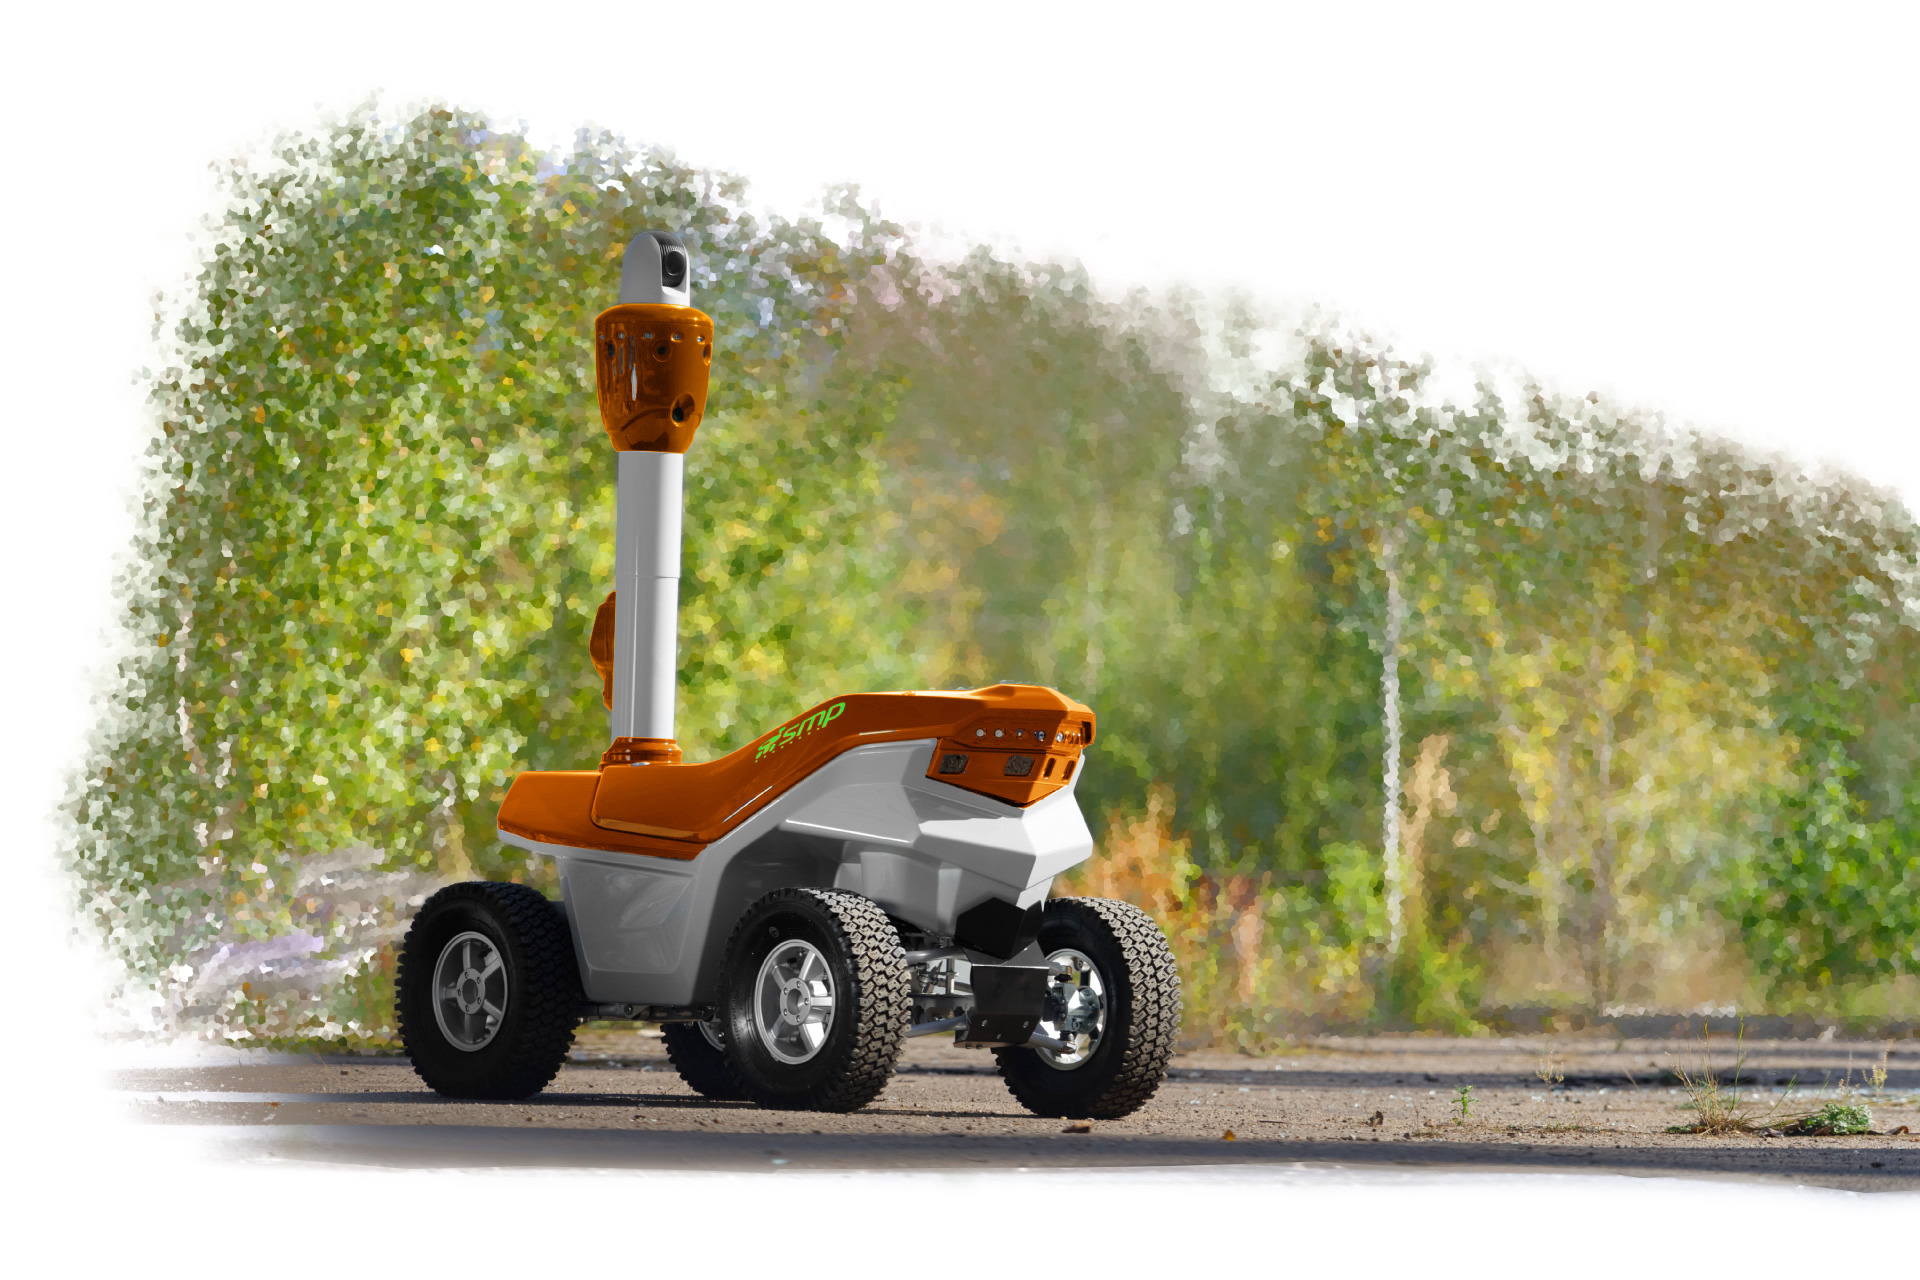
\includegraphics[width=0.618\linewidth]{security_robot_smp.jpg}
    \caption{Robot patrolowy firmy SMP Robotics}
    \label{rys:smp_robot}
\end{figure}
Oferują m.in.: w pełni autonomiczny patrol, sterowanie głosowe, rozpoznawanie twarzy w odległości do 50 metrów i system automatycznego ładowania akumulatorów.

Firma \href{https://robotnik.eu/}{Robotnik} produkuje roboty do różnych zastosowań, w tym model \href{https://robotnik.eu/products/mobile-robots/rb-watcher/}{\textit{RB-Watcher}}.
Jest on przeznaczony do autonomicznego nadzoru wewnątrz budynków, jak i na zewnątrz.
Jego wyposażenie obejmuje bispektralną kamerę, GPS i mikrofon.
Do orientacji w przestrzeni wykorzystuje algorytmy typu SLAM (\textit{Simultaneous localization and mapping}).
Budową przypomina on wspomnianego wyżej robota \ref{smp_robot} od SMP Robotics, ale jest wyraźnie niższy.
Jest on przedstawiony na zdjęciu \ref{rys:robotnik}.
\begin{figure}[!hb]
    \centering 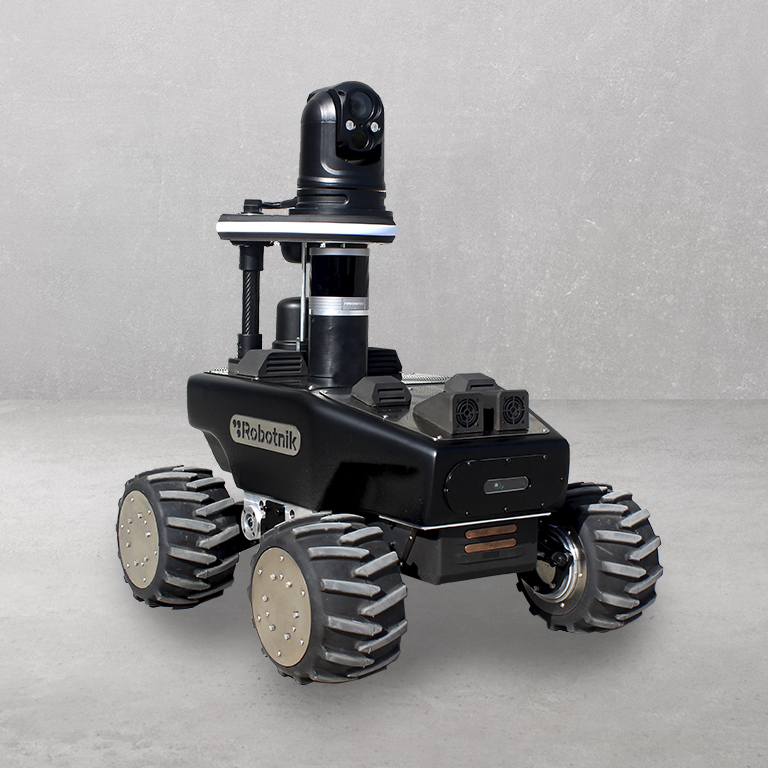
\includegraphics[width=0.618\linewidth]{robotnik.jpg}
    \caption{Robot patrolowy \textit{RB Watcher} firmy Robotnik}
    \label{rys:robotnik}
\end{figure}

Podobne rozwiązanie oferuje firma \href{https://www.knightscope.com/}{Knightscope}.
Na \href{https://www.knightscope.com/products/k5}{stronie internetowej produktu} chwalą się rezultatami zastosowania w postaci:
\begin{itemize}
    \item zmniejszenia liczby zgłaszanych przestępstw o 46\%,
    \item zwiększenia liczby aresztów o 27\%,
    \item zmniejszenia liczby wystawionych mandatów o 68\%.
\end{itemize}
Robot firmy Knightscope wygląda inaczej od przedstawionych wcześniej konkurencyjnych produktów -- widać to na zdjęciu~\ref{rys:knightscope}.
\begin{figure}[!hb]
    \centering 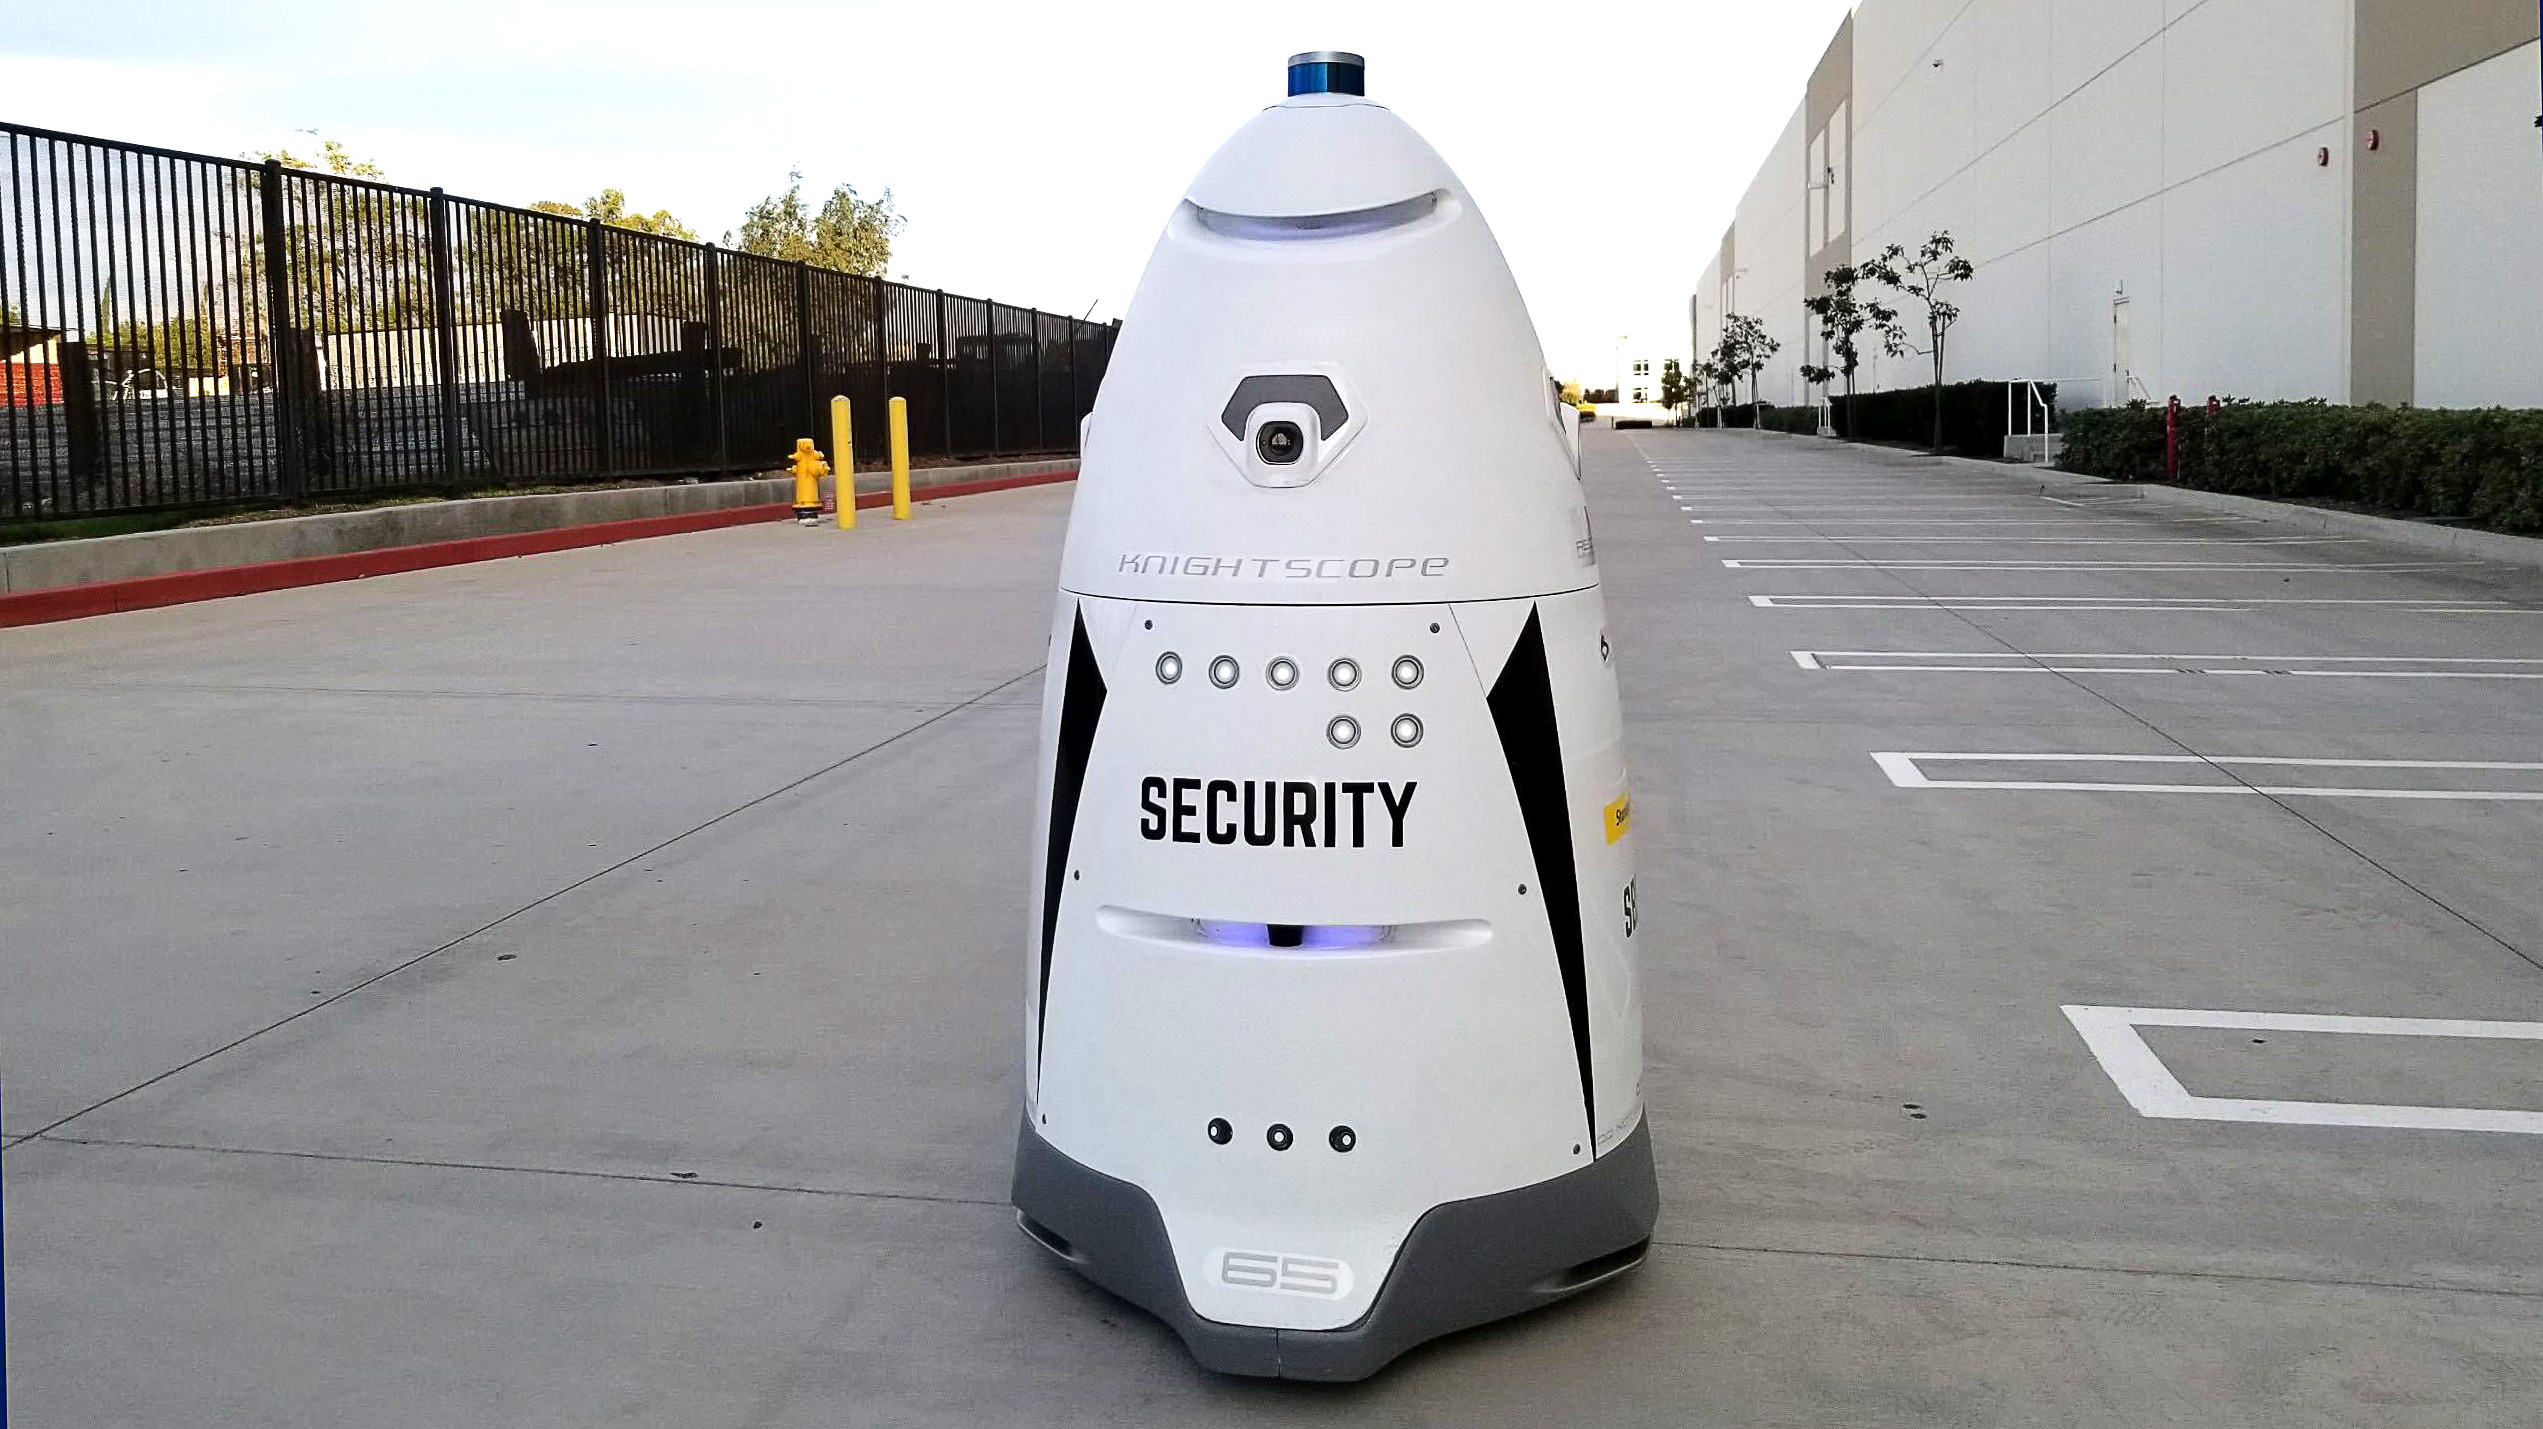
\includegraphics[width=0.618\linewidth]{knightscope.jpg}
    \caption{Robot patrolowy \textit{K5} firmy Knightscope}
    \label{rys:knightscope}
\end{figure}

Mobilne roboty nadzorujące oferują także firmy: Cobalt AI, Running Brains Robotics, Super Droid Robots i inne.

\section{Motywacja}
Obszar mobilnych robotów sprawujących nadzór wydaje się mieć duży potencjał.
Jednocześnie rozwiązania z tej dziedziny nie należą do kanonu narzędzi typowo stosowanych do monitoringu.
Dlatego jest to nisza, która pozostawia w mojej opinii nadal pole do eksploracji.

Zakres tej pracy jest ciekawy ze względu na konieczną fuzję kilku dziedzin inżynierii -- informatyki, elektroniki i mechaniki.
Jako że jednak moją specjalizacją jest informatyka, to najbardziej skupiam się na części związanej z oprogramowaniem robota.
W tym obszarze widzę kilka wyzwań związanych z:
\begin{itemize}
    \item cyberbezpieczeństwem -- zabezpieczenie dostępu do aplikacji webowej, danych użytkowników,
    \item przetwarzaniem danych w czasie rzeczywistym -- przy sterowaniu robotem,
    \item przetwarzaniem multimediów -- strumieniowanie obrazu z kamery do wielu użytkowników.
\end{itemize}
Wyzwania te czynią tę pracę okazją do rozwoju.

% Można też wszystko pisać w jednym pliku ale będzie on duży
%\chapter{Nienudny tytuł dla teorii}
%Można też pisać wszystko w~jednym pliku, tak jak przyzwyczajają do tego gorsze programy, ale wtedy główny plik będzie bardzo duży i~trudniejszy w zarządzaniu.
%
%I~to by było na tyle. Kolejny rozdział jest testem ciągłości numeracji rysunków, wzorów i~innych elementów graficznych. Za nim jest jeszcze rozdział~\ref{ch:podsumowanie} z podsumowaniem, bibliografia, wykazy, spisy i załączniki.

% fragment nieużywany albo jeszcze niedodany można zakomentować
%\input{tekst/teoria}
%\input{tekst/donapisania}
\chapter{Sprzęt}
\section{Cel}
Celami tej części projektu były:
\begin{itemize}
    \item zaplanowanie fizycznej budowy,
    \item zaprojektowanie układu elektronicznego,
    \item wybranie i pozyskanie odpowiednich części,
    \item fizyczne skonstruowanie maszyny.
\end{itemize}

\section{Korpus}
Robot z założenia miał poruszać się na kołach, więc nieodzowne były silniki i podwozie.
Ze względu na brak doświadczenia w konstrukcji pojazdów, zdecydowano się na dobranie gotowego rozwiązania.
Na rynku znaleziono produkt będący zestawem do budowy robota jeżdżącego.
Składa się on z:
\begin{itemize}
    \item dwóch podstaw o rozmiarze 26 x 15 cm,
    \item czterech silników prądu stałego z przekładnią zasilanych napięciem 6V, o momencie obrotowym 0,78 Nm i poborze prądu 0,19 - 1,0 A,
    \item czterech kół z gumowymi oponami o średnicy 6,5 cm,
    \item elementów montażowych -- śrubki, dystanse, nakrętki itp.
\end{itemize}
Zawartość zestawu przedstawiona jest na zdjęciu \ref{rys:podwozie}.
\begin{figure}[!hb]
    \centering 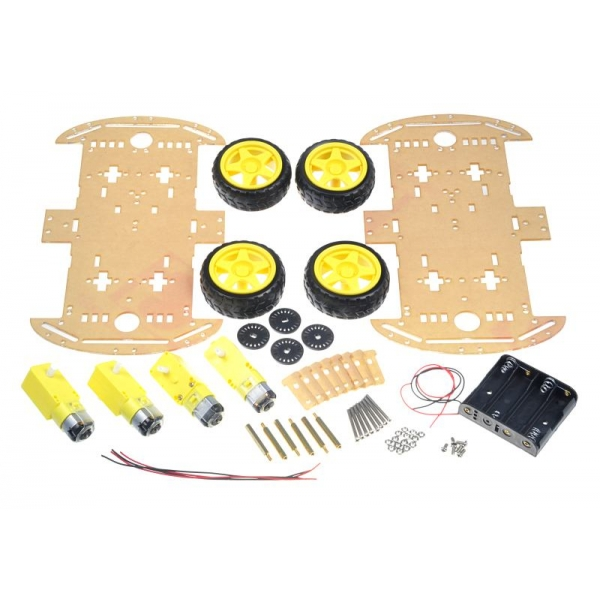
\includegraphics[width=0.618\linewidth]{podwozie.jpg}
    \caption{Gotowa platforma do budowy robota jeżdżącego}
    \label{rys:podwozie}
\end{figure}

Zdecydowano, że biorąc pod uwagę masę konstrukcji, cztery koła jezdne nie są potrzebne i dwa przednie powinny wystarczyć.
Na tył robota przeznaczono obrotowe kółko podporowe.
Dzięki takiemu rozwiązaniu zostaje więcej miejsca na umiejscowienie innych komponentów pomiędzy platformami.
Liczne otwory montażowe w podwoziu zostały wykorzystane do umocowania różnych elementów maszyny.

\section{Elektronika}
Wymagania stawiane względem oprogramowania robota były dosyć wysokie -- strumieniowanie obrazu z kamery, serwowanie aplikacji internetowej, gromadzenie danych.
Jednocześnie potrzebny był interfejs do sterowania silnikami, czy zbierania danych z czujników.
Platformą, która łączy świat pełnoprawnych komputerów i elektroniki jest popularne Raspberry Pi.
Konkretnym modelem wybranym do realizacji tego projektu jest Raspberry Pi 3B+.
Najważniejsze elementy specyfikacji:
\begin{itemize}
    \item wymiary 85 x 56 mm,
    \item 64-bitowy procesor ARM o taktowaniu 1.4GHz oraz 1GB RAM,
    \item karta graficzna Cortex-A53,
    \item karty Wi-Fi i Ethernet,
    \item cztery porty USB 2.0,
    \item porty: 4 x USB, HDMI, RCA, DSI (do wyświetlacza), CSI (do kamery), MicroSD,
    \item 40 pinów GPIO,
    \item napięcie zasilania 5V.
\end{itemize}

Pewną bolączkę stanowił dobór układu zasilania.
W porównaniu do np. Arduino, wadą Raspberry Pi jest mała tolerancja zakresu napięcia zasilania -- +- 5\%.
Ponadto nie posiada układów chroniących przed przepięciami, więc nie jest trudno spalić to urządzenie projektując nieodpowiedni układ lub zwyczajnie będąc nieostrożnym.
Wybrane do projektu silniki elektryczne wymagają wyższego napięcia - 6V.
Dodatkowym utrudnieniem jest charakterystyka silników prądu stałego, które generują zakłócenia na linii zasilania i mają wysoki prąd rozruchowy.

\label{motor_hat}
Z powyższych względów postawiono na gotowy układ projektowany pod Raspberry Pi.
Jest to nakładka \href{https://shop.sb-components.co.uk/products/motor-driver-hat-for-raspberry-pi}{\textit{Motor Driver Hat SKU21789}} od firmy SB Components, która zawiera:
\begin{itemize}
    \item dwukanałowy sterownik silników DC o napięciu 6 - 12 V o poborze prądu do 3A,
    \item generator sygnału PWM o rozdzielczości 12 bitów,
    \item regulator napięcia 5V do zasilania Raspberry Pi,
    \item interfejs komunikacyjny I2C.
\end{itemize}
Komponent ten, zamontowany na Raspberry Pi, przedstawiony jest na zdjęciu \ref{rys:motor_hat}.
\begin{figure}[!hb]
    \centering 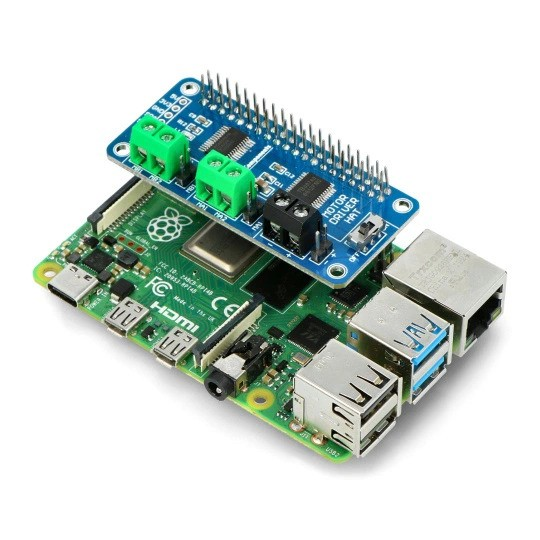
\includegraphics[width=0.618\linewidth]{motor_hat.jpg}
    \caption{Nakładka \textit{Motor Driver Hat SKU21789} na Raspberry Pi}
    \label{rys:motor_hat}
\end{figure}

\section{Zasilanie}
Ze względu na mobilność robota wybrano zasilanie akumulatorowe.
Dzięki zastosowaniu wyżej opisanego układu \ref{motor_hat}, zarówno płytkę Raspberry Pi z peryferiami, jak i silniki można zasilić z tego samego źródła.
Początkowo próbowano zastosować zwykłe baterie AA 1,5V, połączone szeregowo w celu uzyskania źródła napięcia 6V.
To rozwiązanie okazało się nieefektywne -- Raspberry Pi nawet nie było w stanie w całości przejść sekwencji bootowania.
Prawdopodobnie wykorzystane baterie AA nie mały wystarczającej wydajności prądowej.

Ostatecznie zastosowano dwie baterie litowo-jonowe 3,7V typu 18650 o pojemności 3,2 Ah połączone szeregowo.
Mają one wydajność prądową klasy 2C, co oznacza, że można z nich pobierać nawet 6,4 A prądu.
Rozwiązanie to sprostało wyzwaniu jednoczesnego zasilenia mikrokomputera z peryferiami i silników.
Dodatkową stabilność zapewniło podłączenie równolegle dwóch kondensatorów elektrolitycznych o łącznej pojemności 4800 $\mu$F w celu złagodzenia chwilowych spadków napięcia.

\section{Schemat układu}
Połączenie części elektronicznych jest przedstawione na schemacie \ref{rys:schemat}.
\begin{figure}[!hb]
    \centering 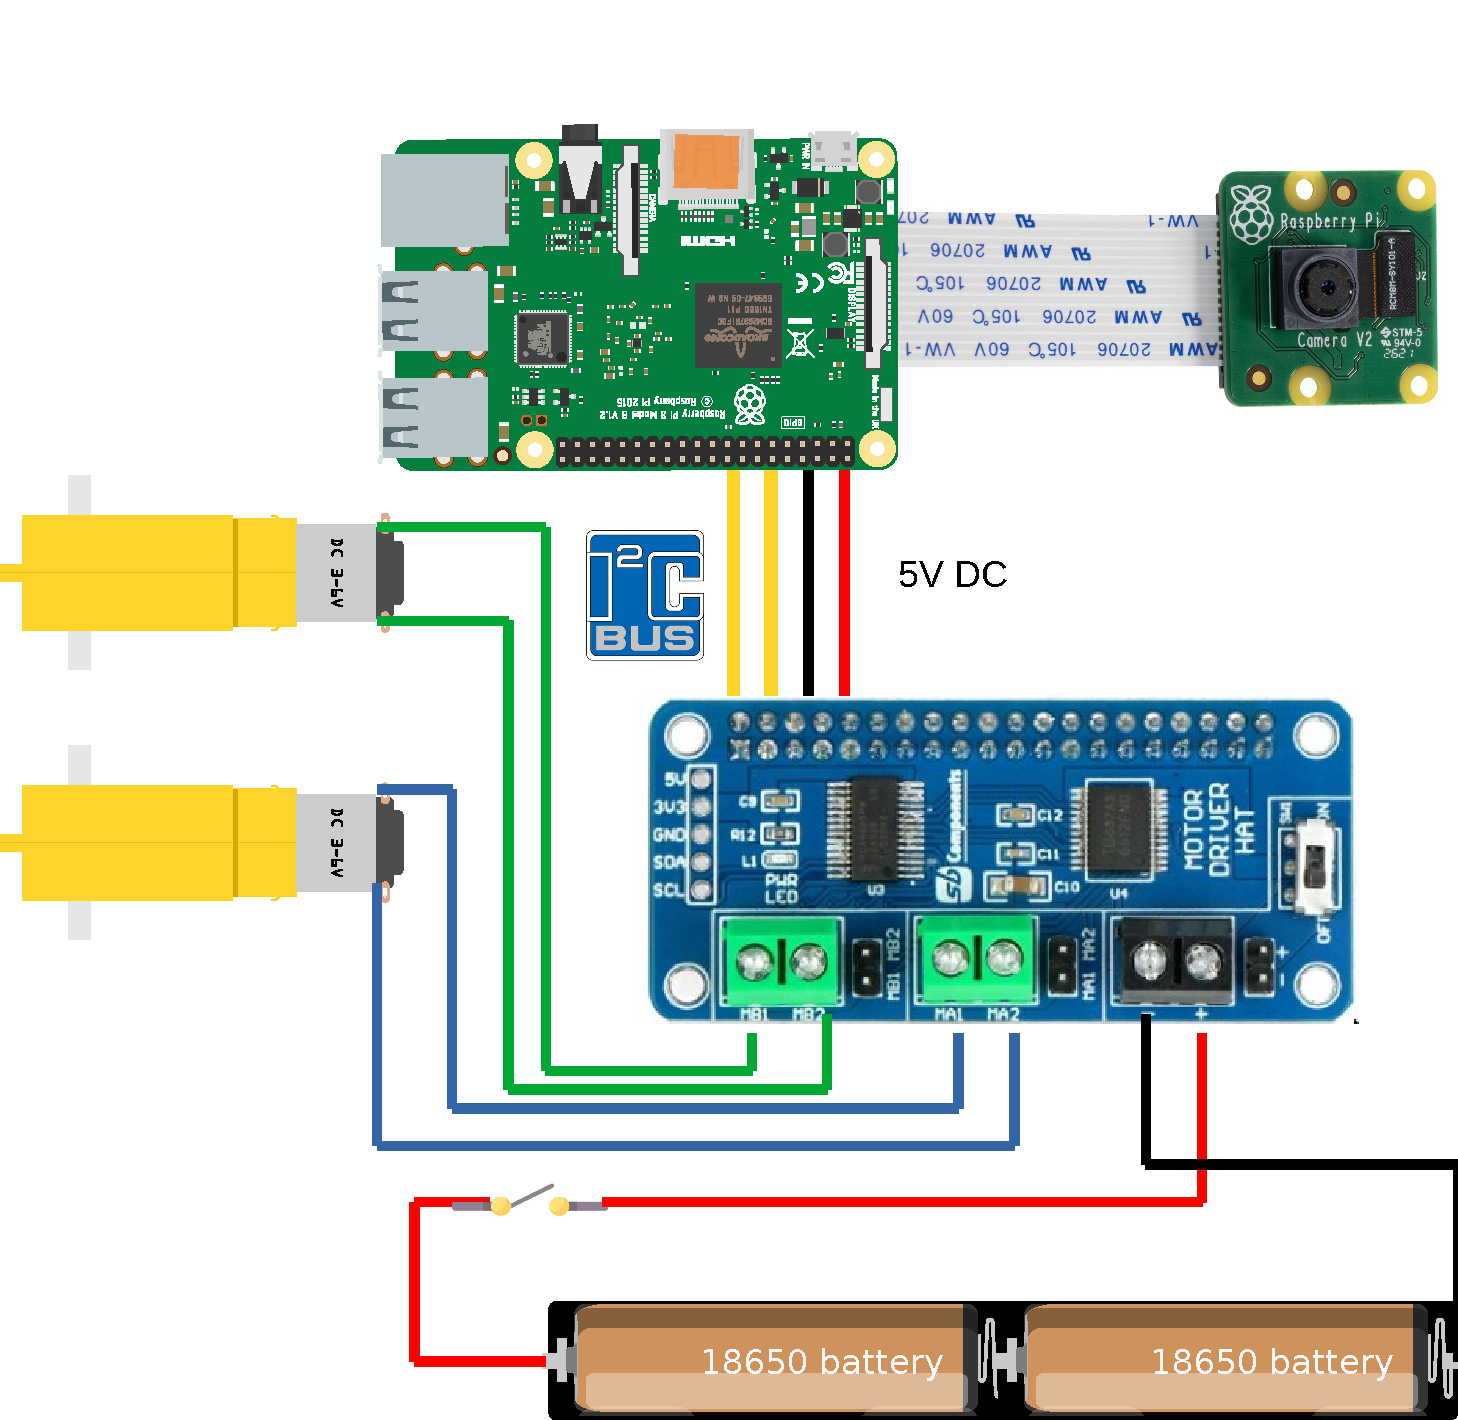
\includegraphics[width=1.0\linewidth]{schemat.pdf}
    \caption{Schemat połączeniowy}
    \label{rys:schemat}
\end{figure}

\section{Złożona konstrukcja}
Po złożeniu podwozia i zamontowaniu połączonych elementów elektronicznych konstrukcja była ukończona.
Efekt końcowy przedstawiają zdjęcia robota z góry \ref{rys:robot_top}, z przodu \ref{rys:robot_front}, z prawego boku \ref{rys:robot_right}, z lewego boku \ref{rys:robot_left} i z tyłu \ref{rys:robot_back}.
\begin{figure}[!hb]
    \centering 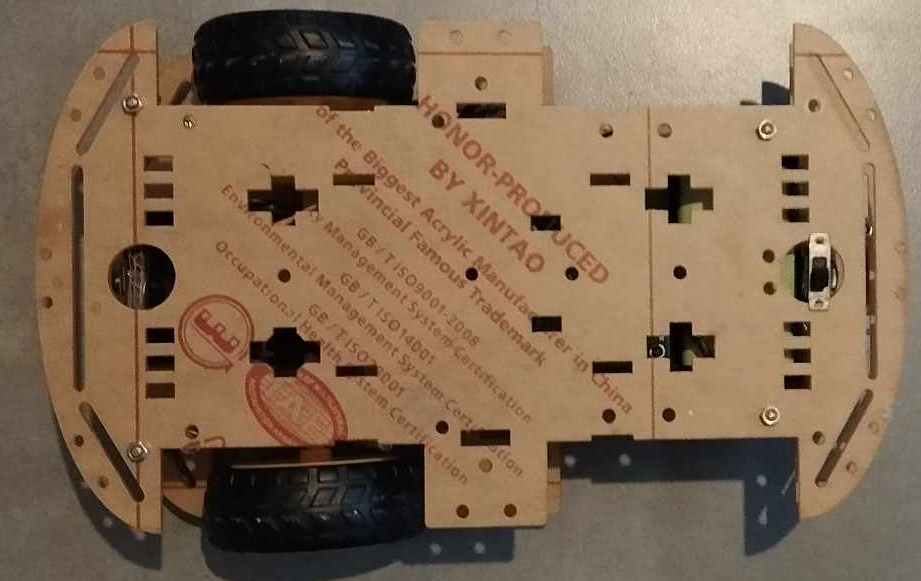
\includegraphics[width=0.618\linewidth]{robot_top.png}
    \caption{Zdjęcie robota z góry}
    \label{rys:robot_top}
\end{figure}
\begin{figure}[!hb]
    \centering 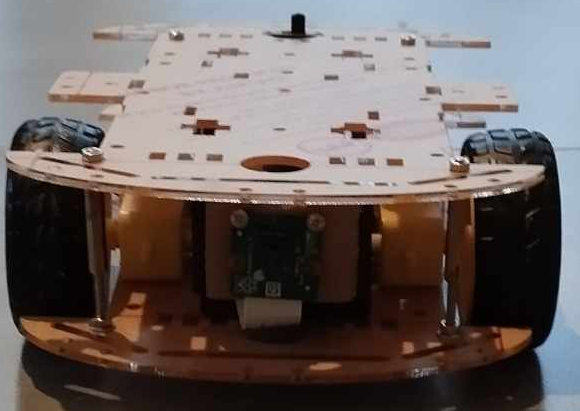
\includegraphics[width=0.618\linewidth]{robot_front.png}
    \caption{Zdjęcie robota z przodu}
    \label{rys:robot_front}
\end{figure}
\begin{figure}[!hb]
    \centering 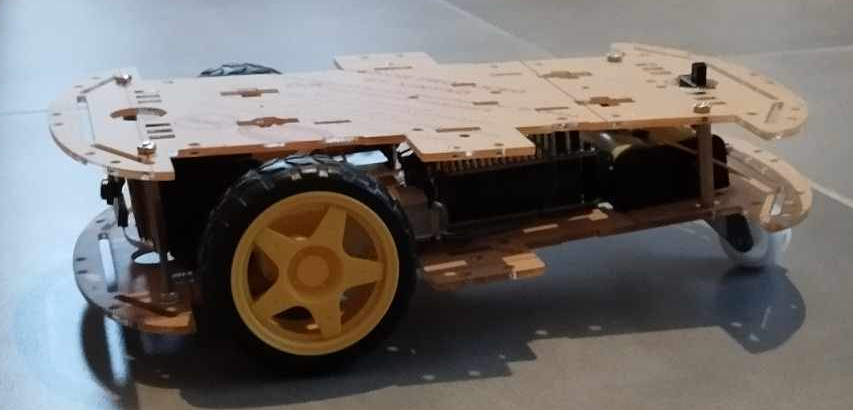
\includegraphics[width=0.618\linewidth]{robot_right.png}
    \caption{Zdjęcie robota z lewej strony}
    \label{rys:robot_left}
\end{figure}
\begin{figure}[!hb]
    \centering 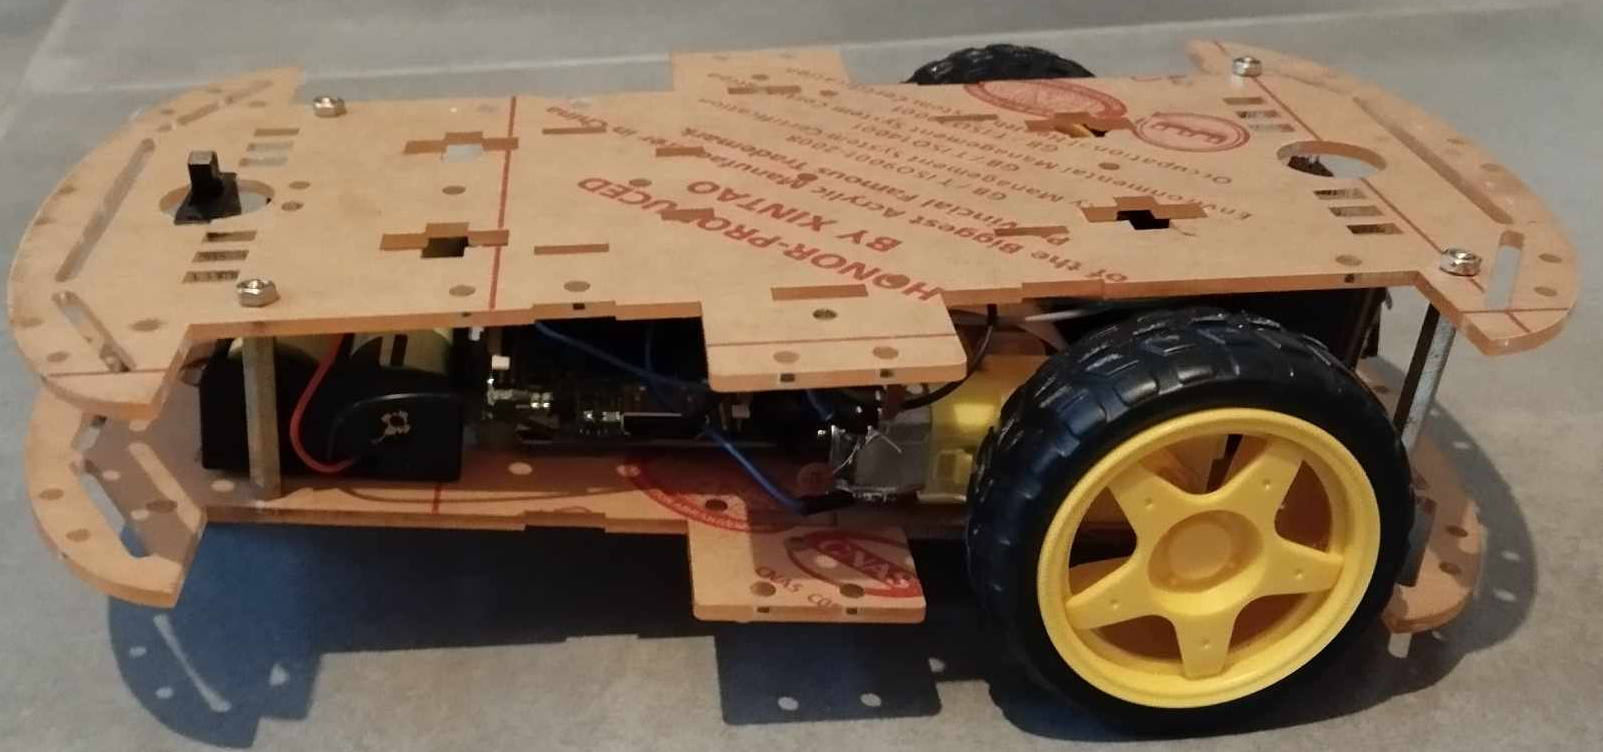
\includegraphics[width=0.618\linewidth]{robot_left.png}
    \caption{Zdjęcie robota z prawej strony}
    \label{rys:robot_right}
\end{figure}
\begin{figure}[!hb]
    \centering 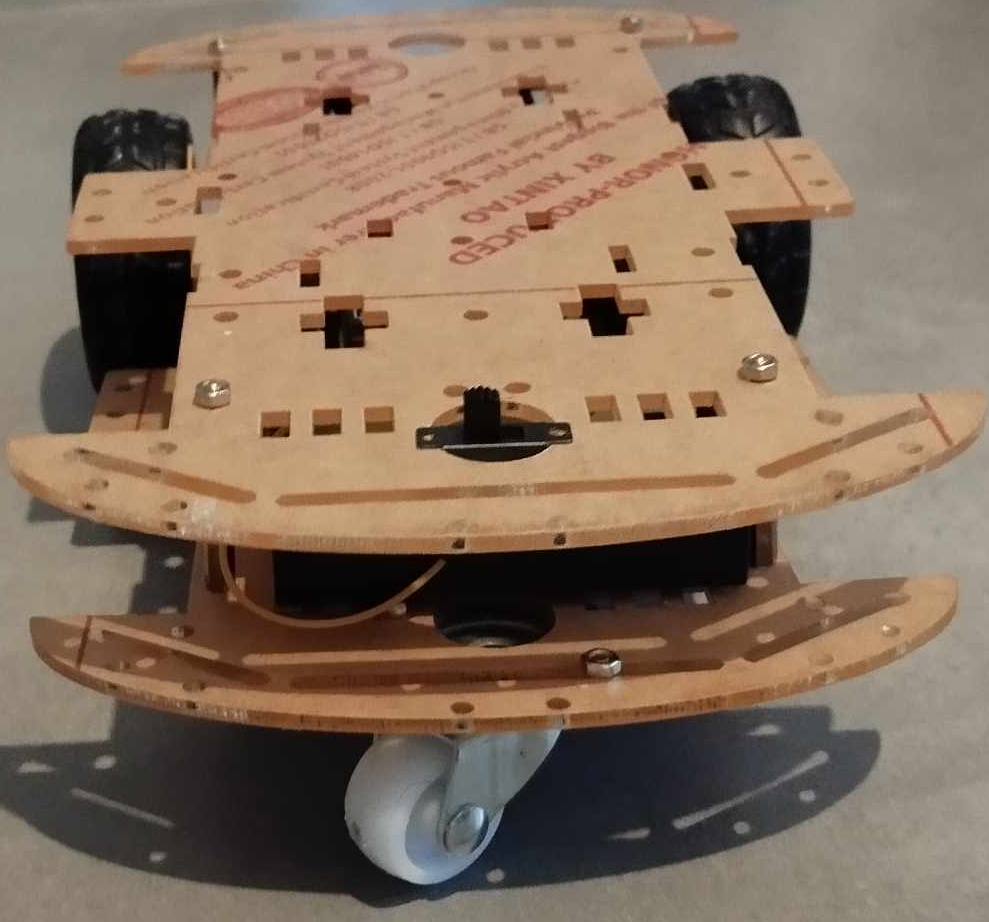
\includegraphics[width=0.618\linewidth]{robot_back.png}
    \caption{Zdjęcie robota z tyłu}
    \label{rys:robot_back}
\end{figure}


\chapter{Oprogramowanie}
\section{Definicja wymagań}
Celem tej części projektu było zaprojektowanie i napisanie oprogramowania robota.
Określono, że będą dwa rodzaje aktorów ludzkich wchodzących w interakcje z systemem:
\begin{itemize}
    \item administrator -- jest tylko jeden i ma dostęp do wszystkich ustawień i zarządzania pozostałymi użytkownikami;
    \item pracownik ochrony -- ma dostęp do kluczowych funkcjonalności;
\end{itemize}
Funkcjonalności, jakie ma posiadać system zostały zdefiniowane na diagramie przypadków użycia \ref{rys:usecases}.
\begin{figure}[!hb]
    \centering 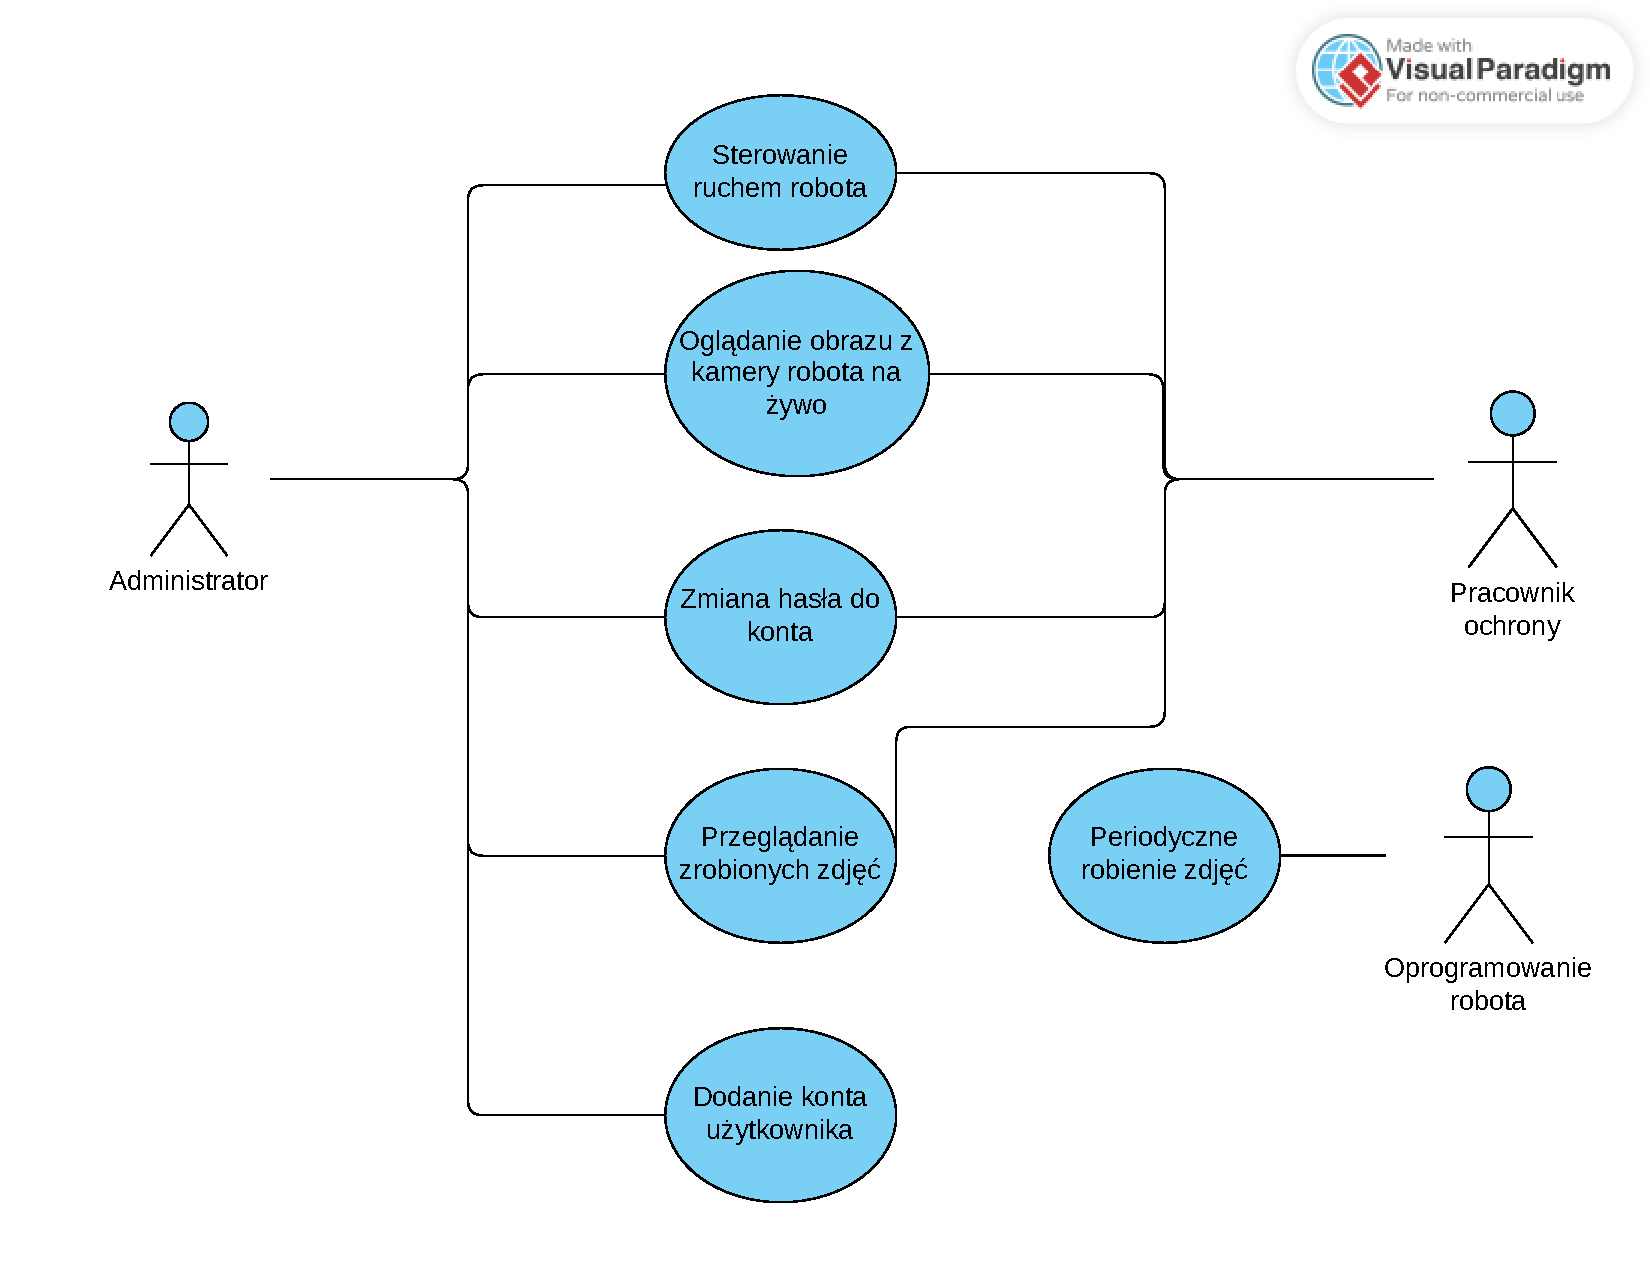
\includegraphics[width=1.0\linewidth]{robot_usecases.pdf}
    \caption{Diagram przypadków użycia}
    \label{rys:usecases}
\end{figure}

\section{Architektura systemu}
Zdecydowano się na interfejs użytkownika w formie aplikacji przeglądarkowej (webowej).
Rozwiązanie to pozwala na dostęp do systemu bez instalacji żadnego oprogramowania.
Ponadto taka forma aplikacji pozwala na dostęp przez szeroką gamę urządzeń końcowych -- komputery, smartfony, tablety itp.

Zgrubny podział aplikacji jest na:
\begin{itemize}
    \item Frontend \\
    Aplikacja uruchamiana w przeglądarce użytkownika.
    Prezentuje dane przychodzące z robota użytkownikowi.
    Przesyła do backendu dane pochodzące od użytkownika.
    \item Backend \\
    Aplikacja działająca na sprzęcie robota.
    Wysyłająca dane do frontendu i przetwarzająca przychodzące dane.
    Steruje zachowaniem robota.
\end{itemize}

Na backendzie ze względu na różnorodną i wielowarstwową funkcjonalność aplikacji zdecydowano się na architekturę mikroserwisową.
Wysokopoziomowa komunikacja modułów między sobą ukazana jest na diagramie komponentów \ref{rys:components}.
\begin{figure}[!hb]
    \centering 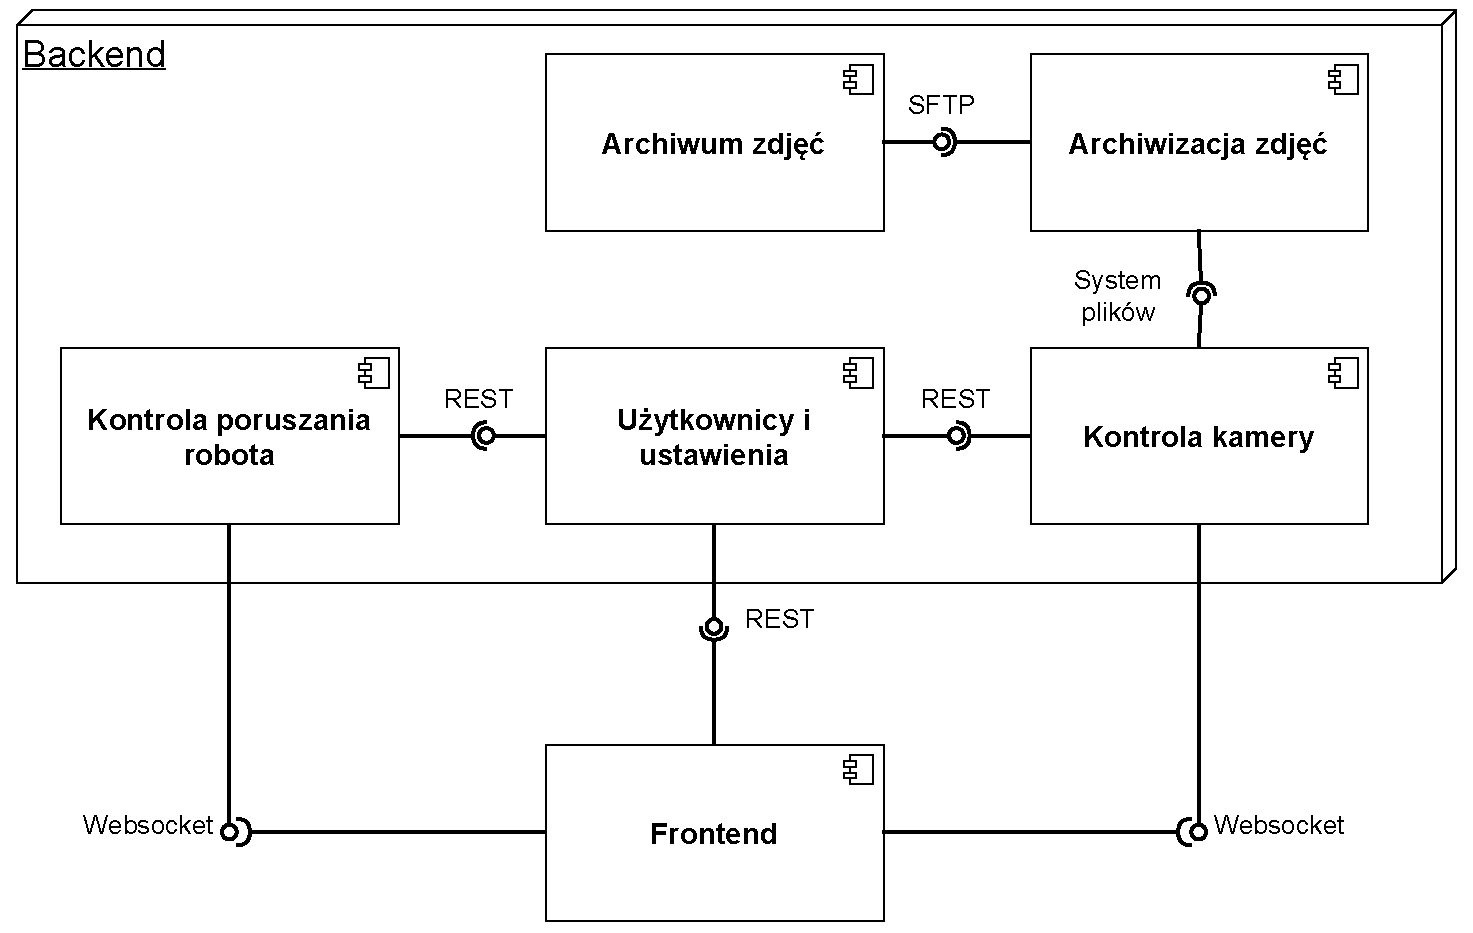
\includegraphics[width=1.0\linewidth]{robot_components.pdf}
    \caption{Diagram komponentów}
    \label{rys:components}
\end{figure}

\section{Wdrożenie}
Wdrożona aplikacja ma działać na sprzęcie samego robota i na urządzeniach końcowych użytkowników.
Wykorzystując możliwości minikomputera Raspberry Pi stawiany jest na nim serwer backendu i frontendu.
Jedynym wykorzystaniem zewnętrznej infrastruktury jest zewnętrzny serwer na pliki, gdzie archiwizowane są zdjęcia.
Architektura wdrożeniowa przedstawiona jest na schemacie \ref{rys:deploy}.

We wdrożeniu wszystkie moduły backendowe są schowane za reverse proxy, które stanowi odpowiednio skonfigurowany serwer HTTP \href{https://nginx.org/}{\textit{nginx}}.
Do uruchamiania całej aplikacji napisany został skrypt w bashu.
Skrypt ten z kolei jest uruchamiany przez specjalnie napisany serwis \textit{systemd}\footnote{\textit{systemd} to menadżer systemu i usług w wielu dystrybucjach systemu operacyjnego GNU/Linux.}.

Jeśli chodzi o architekturę sieciową, to robot jest połączony do internetu przez bezprzewodową sieć Wi-Fi.
Ponadto, administrator może podłączyć maszynę do wirtualnej sieci prywatnej.
\href{https://www.zerotier.com/}{\textit{ZeroTier}} jest popularnym tego typu oprogramowaniem wykorzystanym w tym projekcie.
Dzięki temu rozwiązaniu użytkownicy robota mogą korzystać z systemu robota w jakimkolwiek miejscu z dostępem do internetu.
Jednocześnie \textit{ZeroTier} szyfruje cały ruch sieciowy od końca do końca, co gwarantuje bezpieczeństwo i prywatność.
\begin{figure}[!hb]
    \centering 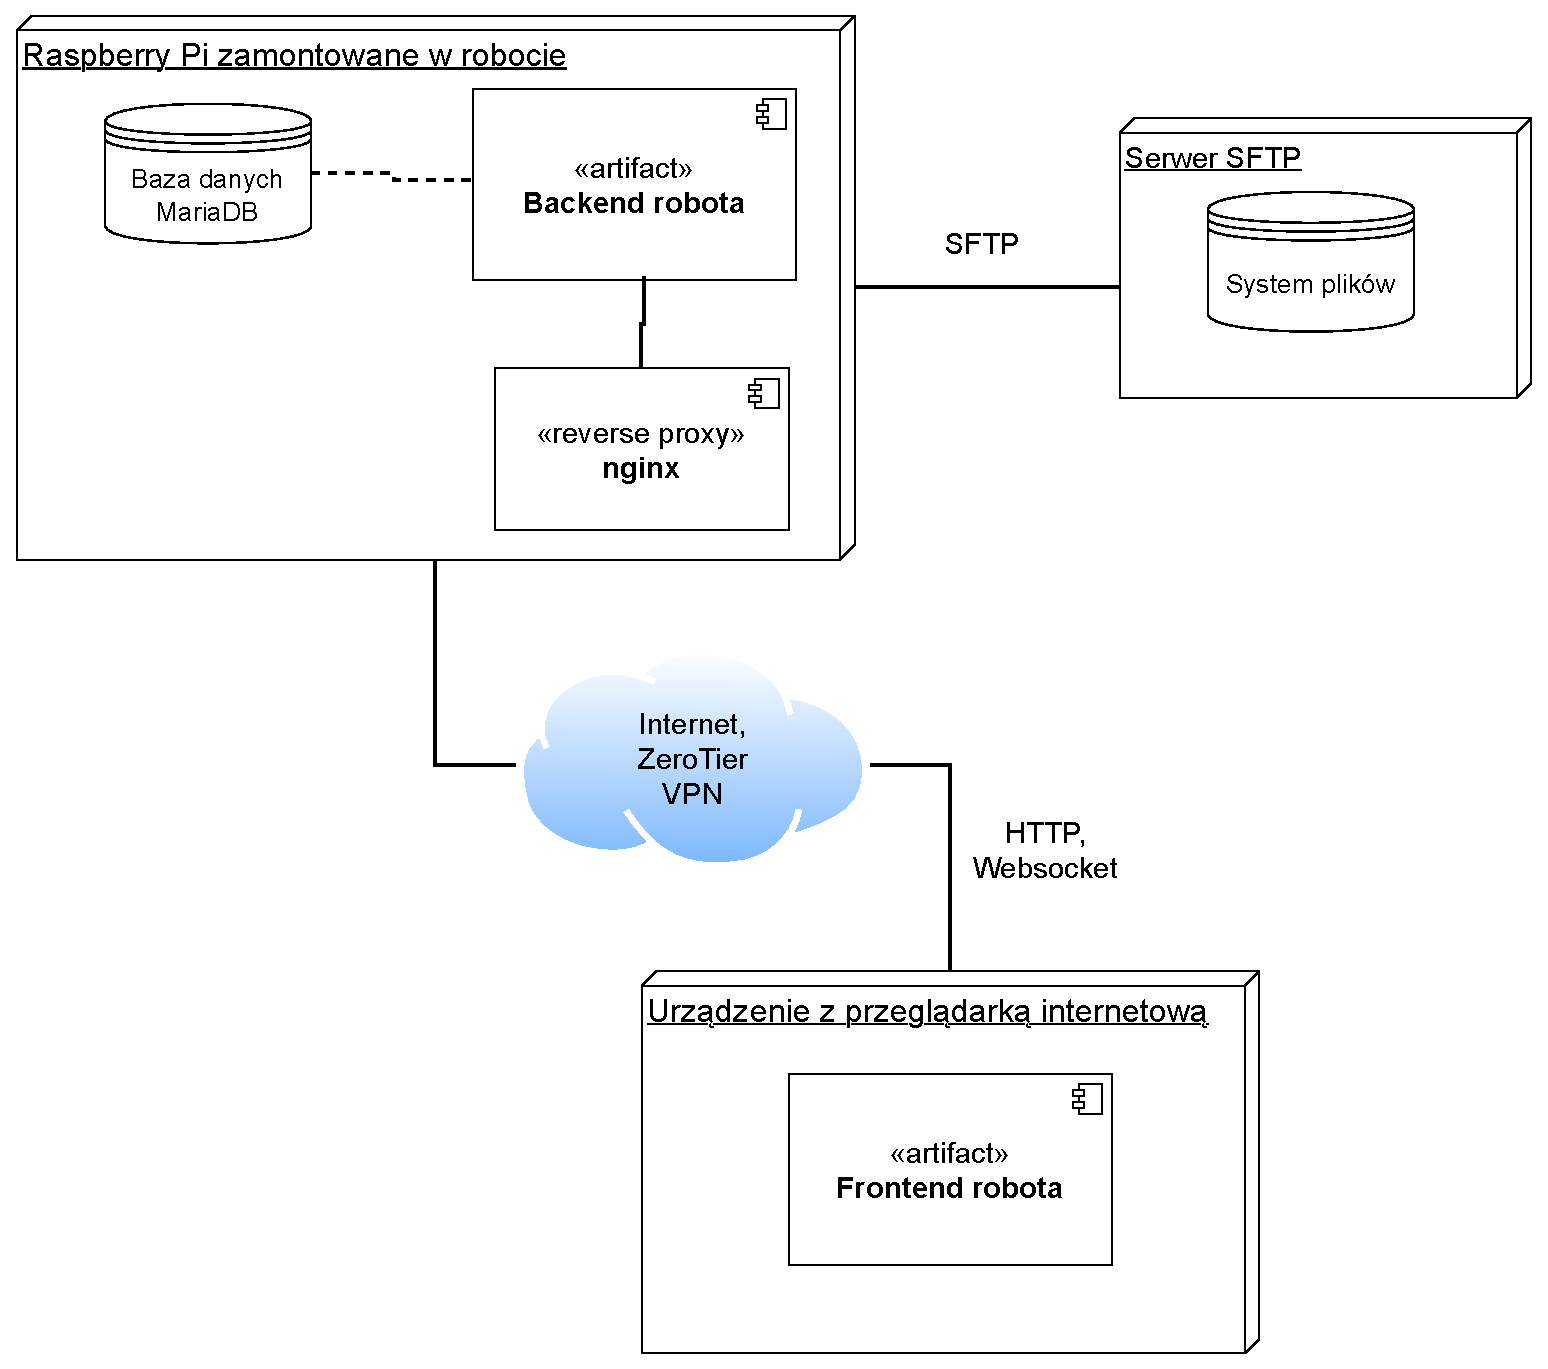
\includegraphics[width=1.0\linewidth]{robot_deploy.pdf}
    \caption{Diagram wdrożenia}
    \label{rys:deploy}
\end{figure}




\chapter{Testy}
\section{Testy oprogramowania}
W czasie wytwarzania oprogramowanie było testowane przez 3 rodzaje testów automatycznych:
\begin{itemize}
    \item jednostkowe - sprawdzające poprawność logiki kodu,
    \item integracyjne - weryfikujące poprawność zachowania poszczególnych mikroserwisów,
    \item end-to-end - symulujące zachowanie użytkownika.
\end{itemize}

Testy integracyjne serwisu użytkowników i ustawień \ref{main_backend} zostały napisane z wykorzystaniem biblioteki \href{https://pypi.org/project/Flask-Testing/}{\textit{Flask testing}}.
W przypadku serwisów napisanych za pomocą frameworka FastAPI wykorzystano jego wbudowane biblioteki do testowania.

Testy end-to-end zostały zbudowane za pomocą nowoczesnego narzędzia przeznaczonego do tego celu -- \href{https://www.cypress.io/}\textit{Cypress}.
Użyto języka Javascript.

Ponadto zostały przeprowadzone szerokie testy manualne, których scenariusze zostały dopasowane do przypadków użycia zdefiniowanych w wymaganiach \ref{rys:usecases}.
Aby można było testować oprogramowanie bez uruchamiania całego robota, klasy odpowiadające za sterowanie silnikami i zbieranie obrazu z kamery zostały zastąpione klasami pozorowanymi (ang. \textit{mock}).

\section{Testy robota}
Po ukończeniu budowy sprzętu i oprogramowania przystąpiono do sprawdzania działania całego rozwiązania.
Powtórzono napisane wcześniej automatyczne testy end-to-end, tym razem na w pełni wdrożonym systemie.

Głównym przypadkiem użycia robota jest zdalne sterowanie przez internet.
Zostało to przetestowane przez autora projektu i osobę postronną w następujących scenariuszach:

Scenariusz 1 -- sterowanie robotem w sieci lokalnej.
Operator był podłączony na komputerze do tej samej sieci bezprzewodowej Wi-Fi, co robot.
Średnie opóźnienie (ping) wynosił ok. 15 ms.

Scenariusz 2 -- sterowanie robotem przez internet na dobrym łączu.
Operator był podłączony na komputerze do innej sieci niż robot.
Sieć robota i operatora były połączone światłowodem.
Średnie opóźnienie (ping) wynosił ok. 30 ms.

Scenariusz 3 -- sterowanie robotem przez internet na łączu mobilnym.
Operator łączył się z robotem na telefonie korzystając z bezprzewodowej sieci komórkowej 4G LTE.
Średnie opóźnienie (ping) wynosił ok. 60 ms.

Robot był umieszczony na płaskiej podłodze w biurze, gdzie były typowe dla tego środowiska przeszkody.

Subiektywne odczucia po testach były takie, że robot jest w stanie spełniać swoją rolę.
Jednak sterowanie nie było łatwe i wymagało przyzwyczajenia.
Często ruchy robota wydawały się zbyt gwałtowne.
Zmniejszenie parametru maksymalnej mocy silników pomagało w płynniejszej jeździe.
W scenariuszu 3 trochę przeszkadzało opóźnienie transmisji obrazu z kamery, szczególnie, że jest on ograniczony do 10 klatek na sekundę.

Robot nie radzi sobie z pokonywaniem wysokich progów i innych podobnych przeszkód.
Jeszcze większym oczywistym problemem są drzwi lub schody.

Kolejnym testem było zmierzenie zużycia energii elektrycznej.
W tym celu zmierzono natężenie prądu pobieranego z akumulatorów multimetrem.
Stwierdzono, że w bezruchu pobierane jest ok. 0.35 A.
W trakcie ruchu silników z wypełnieniem PWM 50\% natężenie wynosiło ok. 0.7 A.
Na podstawie tych danych i pojemności akumulatorów 3.4 Ah obliczono, że bez jazdy robot może działać przez około 8 godzin.

\chapter{Podsumowanie}
\label{ch:podsumowanie}
\section{Realizacja celu}
Cel pracy uznaje się za zrealizowany.
Efektem końcowym jest mobilny robot z kamerą, który jest sterowany przez stronę internetową.
Posiada on założone funkcjonalności, które czynią go zdatnym do wykorzystania do monitoringu budynku.

Trzeba jednak przyznać, że część sprzętowa została zrealizowana tanim kosztem i ma charakter raczej prototypowy.
Przez to, praktyczne zastosowanie robota jest ograniczone.
Na przykład, słabo radzi sobie z pokonywaniem przeszkód.

Za to zbudowany system informatyczny ma wiele mocnych stron i jest gotowy do dalszego rozwoju.
Komunikacja między stroną internetową a robotem działa sprawnie, a interfejs jest intuicyjny i responsywny.
Architektura systemu jest modularna i pozwala na łatwe dodawanie nowych funkcjonalności.

\section{Możliwości rozwoju}
W przyszłości można rozwinąć projekt w kilku kierunkach:
\begin{itemize}
    \item Dodanie elementów autonomiczności.
    Robot mógłby samodzielnie patrolować zadany obszar lub ścieżkę.
    Można by wykorzystać np. algorytmy typu SLAM do mapowania otoczenia na podstawie obrazu z kamery.
    Dużo wartości dodałaby funkcjonalność samodzielnego dokowania do stacji ładowania.
    \item Dołożenie większej liczby czujników.
    Wartość robota jako urządzenia nadzorującego urosłaby, gdyby mógł on zbierać więcej informacji o otoczeniu.
    Można by dodać kamery termowizyjne, mikrofony.
    \item Zwiększenie mobilności.
    Robot mógłby być bardziej wszechstronny, gdyby mógł pokonywać większe przeszkody.
    \item Wydłużenie czasu pracy.
    Obecnie robot może działać przez około 8 godzin.
    Można tę wartość łatwo zwiększyć przez zastosowanie większych akumulatorów.
\end{itemize}


    % Bibliografia - musi być
    % Bibliography - must exist
    \bibliografia

    % Strony końcowe - można zakomentować, jeśli zbędne
    % Additional pages - comment out if not needed
    
    % Spis rysunków
    \listoffigures
\end{document}
%%%%%%%%%%%%%%%%%%%%%%%%%%%%%%%%%%%%%%%%%%%%%%%%%%%%%%%%%%%%%%%%%%%%%%%%%%%

